\documentclass{article}
  \usepackage{amsmath}
  \usepackage{amssymb}
  \usepackage{graphicx}
  \usepackage{float}
  \usepackage{setspace}
  \usepackage{verbatim}
\topmargin=-1.2cm \oddsidemargin=0.1cm \evensidemargin=0.1cm
\textwidth=16 true cm \textheight=23 true cm

\font\euler=EUSM10 \font\eulers=EUSM7

\begin{document}
\title{ECON 3160 Game Theory \\Assignment $3^{\text{rd}}$}
\author{{\normalsize Leonard Sheng(SHENG, Hao), 1155035947, via \LaTeX}}
\date{\today}

\maketitle

\def \Pr{{\rm Pr}}

\baselineskip 0.6cm
\begin{description}
    \item[Problem(a)-(d):]{\bf Answer:}\\
    {\bf Background Story: Going to university}\\
    You, Barbara and Chris are classmates when you were in high school in mainland China. Now you have to select the university: There are two top universities in Beijing, namely, Peking University(PKU) and Tsinghua University(THU); two top universities in Hong Kong, The Chinese University of Hong Kong and Hong Kong University(HKU); and two perfect university next to Boston, Yale and Harvard. And since you are all super-duper excellent among peers, no university will turn down your application. However, your parents only allow you to select universities in Beijing, because they want to see you at weekend, otherwise they will not sponsor you. Barbara's parents ask her to choose a Hong Kong university because they want her to learn some Cantonese. Chris' parents ask him to go to university near Boston because they want him to have oversea education background, and he has an aunt living in Boston. In this case, no matter what your and your friends' choices are, you can hardly meet again in the university campus. Let's assume no matter what the choice combination, each of you will get utility of ZERO. So, we can draw a belief diagram arbitrarily since every choice is rational and every belief hierarchy will express common belief in rationality.\\
    {\bf (a):}
    The belief diagram:
    \begin{center}
                    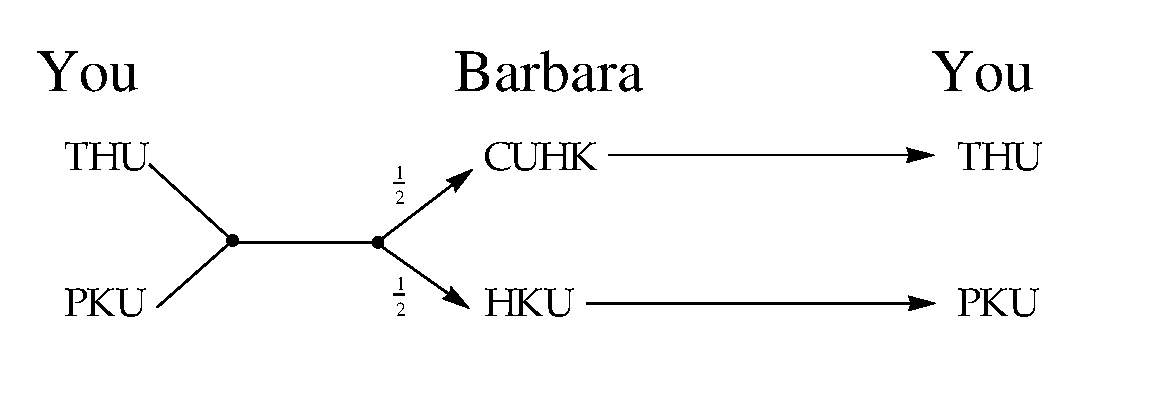
\includegraphics[angle=0, width=0.5\textwidth]{ECON3160A3P1}\\
    \end{center}
    \begin{comment}
    The epistemic model:
    \begin{center}
        \begin{tabular}{cr}
        \hline
        \hline
        \multicolumn{ 1}{c}{{\bf Type}} &          $T_1=\left\{t_1^{\text{THU}},t_1^{\text{PKU}}\right\}$ \\

        \multicolumn{ 1}{c}{{\bf }}  &          $T_2=\left\{t_2^{\text{CUHK}},t_2^{\text{HKU}}\right\}$ \\
        \hline
        \multicolumn{ 1}{c}{{\bf Belief of You}} &         $b_1\left(t_1^{\text{THU}}\right)=\frac{1}{2}\left(CUHK,t_2^{\text{CUHK}}\right)+\frac{1}{2}\left(HKU,t_2^{\text{HKU}}\right)$ \\

        \multicolumn{ 1}{c}{{\bf }} &         $b_1\left(t_1^{\text{PKU}}\right)=\frac{1}{2}\left(CUHK,t_2^{\text{CUHK}}\right)+\frac{1}{2}\left(HKU,t_2^{\text{HKU}}\right)$ \\
\\


        \multicolumn{ 1}{c}{{\bf Belief of Barbara}} &         $b_2\left(t_2^{\text{CUHK}}\right)=\left(THU,t_1^{\text{THU}}\right)$ \\

        \multicolumn{ 1}{c}{{\bf }} &         $b_2\left(t_2^{\text{HKU}}\right)=\left(PKU,t_1^{\text{PKU}}\right)$ \\
        \hline
        \hline
        \end{tabular}
    \end{center}
    \end{comment}
    It's easy to check that your type $t_1^{\text{THU}}$ meets the requirements. It doesn't have a simple belief hierarchy. \\\\
    {\bf (b):}
    The belief diagram:
    \begin{center}
                    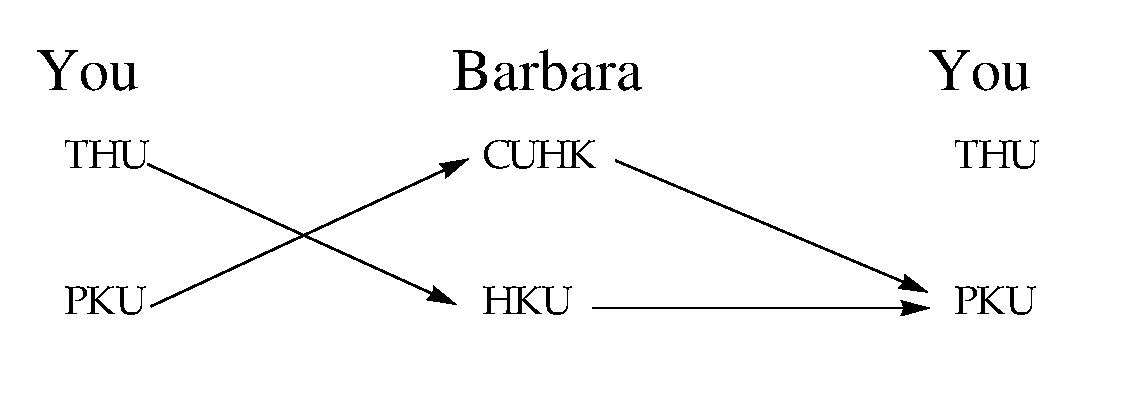
\includegraphics[angle=0, width=0.5\textwidth]{ECON3160A3P2}\\
    \end{center}
    It's easy to check that your type $t_1^{\text{THU}}$ meets the requirements. It doesn't have a simple belief hierarchy. \\\\
    {\bf (c):}
    The belief diagram:
    \begin{center}
                    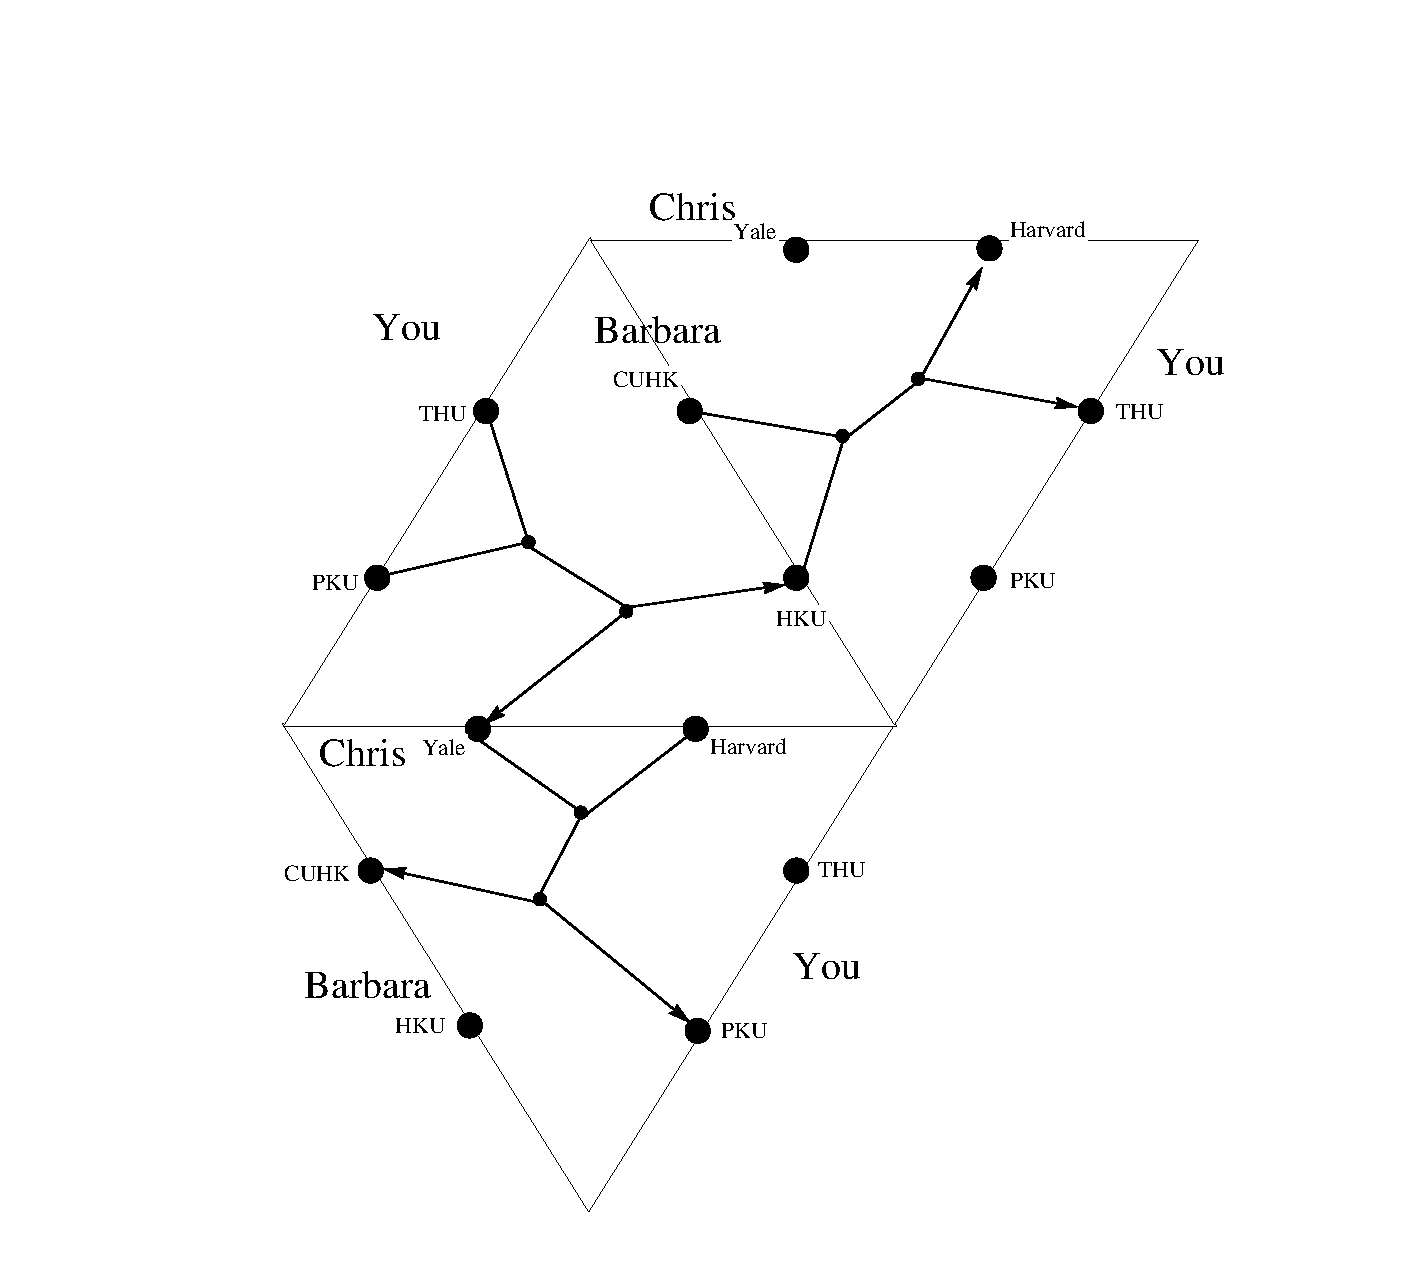
\includegraphics[angle=0, width=0.8\textwidth]{ECON3160A3P3}\\
    \end{center}
    It's easy to check that your type $t_1^{\text{THU}}$ meets the requirements. It doesn't have a simple belief hierarchy. \\\newpage
    {\bf (d):}
    We only construct YOUR belief hierarchies. But it's enough to make sure that the game meets the requirement.\\
    The belief diagram:
    \begin{center}
                    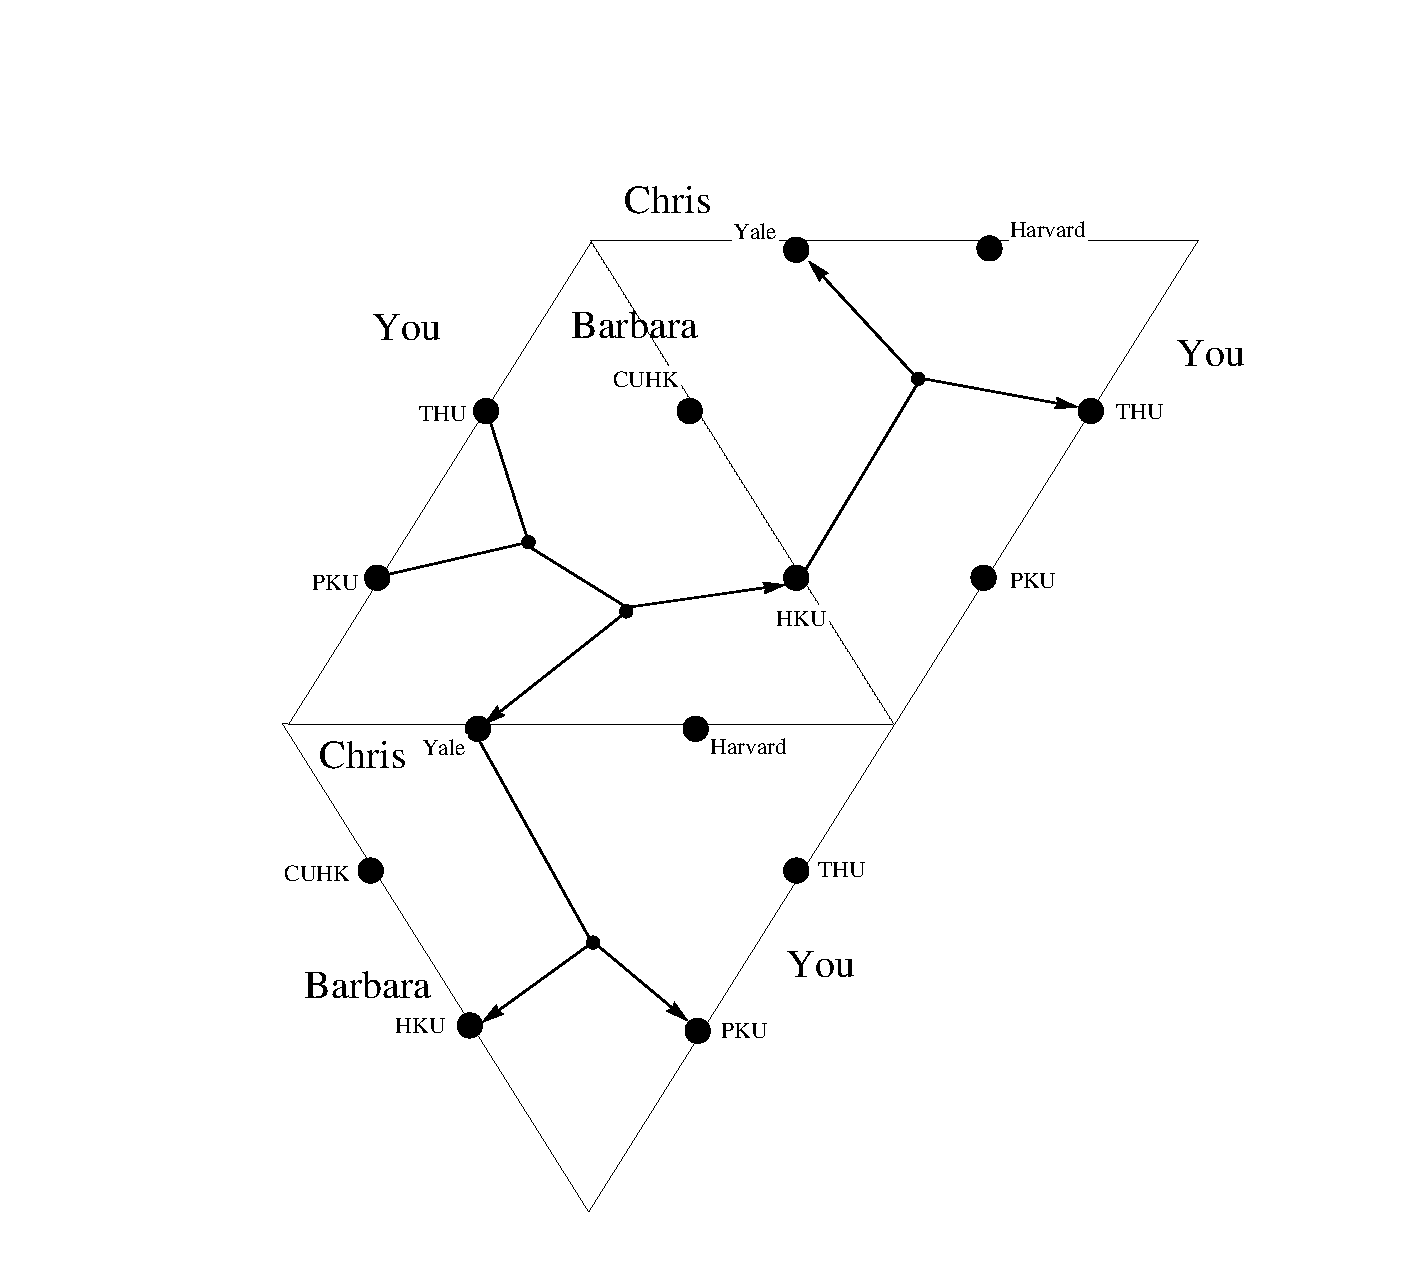
\includegraphics[angle=0, width=0.8\textwidth]{ECON3160A3P4}\\
    \end{center}
    It's easy to check that your type $t_1^{\text{THU}}$ meets the requirements. It doesn't have a simple belief hierarchy. \\\\
    \item[Problem(e), 4.4:]{\bf Answer:}\\
    We denote $I$ for the choice of writing Iceland on the paper, and $S$ for the choice of writing Spain on the paper.\\\newpage
    {\bf a)}
    The belief diagram:
    \begin{center}
                    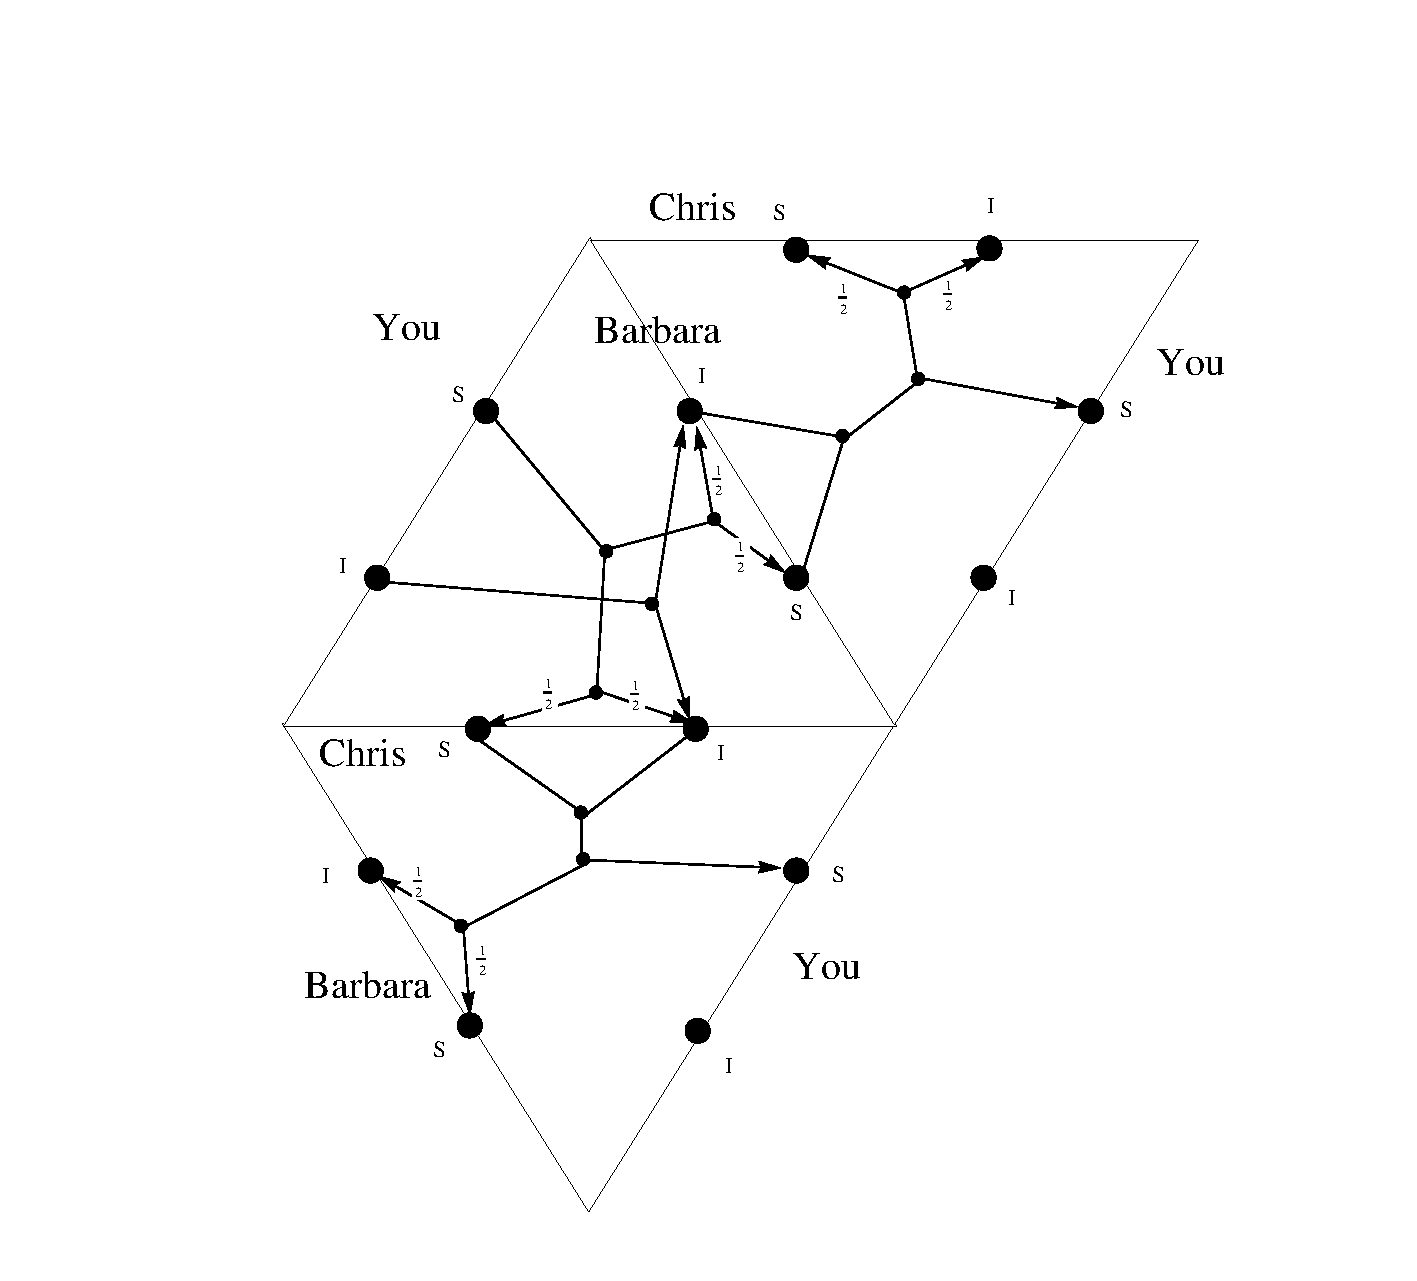
\includegraphics[angle=0, width=0.8\textwidth]{ECON3160A3P5}\\
    \end{center}
       The epistemic model:
    \begin{center}
        \begin{tabular}{cl}
        \hline
        \hline
        \multicolumn{ 1}{c}{{\bf Type}} &          $T_1=\left\{t_1^{\text{I}},t_1^{\text{S}}\right\}$ \\

        \multicolumn{ 1}{c}{{\bf }} &          $T_2=\left\{t_2^{\text{I}},t_2^{\text{S}}\right\}$ \\

        \multicolumn{ 1}{c}{{\bf }} &          $T_3=\left\{t_3^{\text{I}},t_3^{\text{S}}\right\}$ \\
        \hline
        \multicolumn{ 1}{c}{{\bf Belief of You}} &         $b_1\left(t_1^{\text{I}}\right)=\left(\left(I,t_2^I\right),\left(I,t_3^I\right)\right)$\\

        \multicolumn{ 1}{c}{{\bf }} &         $b_1\left(t_1^{\text{S}}\right)=\left(\left(\left(\frac{1}{2}\right)\cdot \left(I,t_2^I\right)+\left(\frac{1}{2}\right)\cdot \left(S,t_2^S\right)\right),\left(\left(\frac{1}{2}\right)\cdot \left(I,t_3^I\right)+\left(\frac{1}{2}\right)\cdot \left(S,t_3^S\right)\right)\right)$ \\\\

        \multicolumn{ 1}{c}{{\bf Belief of Barbara}} &         $b_2\left(t_2^{\text{I}}\right)=\left(\left(S,t_1^S\right),\left(\left(\frac{1}{2}\right)\cdot \left(I,t_3^I\right)+\left(\frac{1}{2}\right)\cdot \left(S,t_3^S\right)\right)\right)$\\

        \multicolumn{ 1}{c}{{\bf }} &         $b_2\left(t_2^{\text{S}}\right)=\left(\left(S,t_1^S\right),\left(\left(\frac{1}{2}\right)\cdot \left(I,t_3^I\right)+\left(\frac{1}{2}\right)\cdot \left(S,t_3^S\right)\right)\right)$ \\\\

        \multicolumn{ 1}{c}{{\bf Belief of Chris}} &         $b_3\left(t_3^{\text{I}}\right)=\left(\left(S,t_1^S\right),\left(\left(\frac{1}{2}\right)\cdot \left(I,t_2^I\right)+\left(\frac{1}{2}\right)\cdot \left(S,t_2^S\right)\right)\right)$ \\

        \multicolumn{ 1}{c}{{\bf }} &         $b_3\left(t_3^{\text{S}}\right)=\left(\left(S,t_1^S\right),\left(\left(\frac{1}{2}\right)\cdot \left(I,t_2^I\right)+\left(\frac{1}{2}\right)\cdot \left(S,t_2^S\right)\right)\right)$ \\

        \hline
        \hline
        \end{tabular}
    \end{center}
    Both of your choice $I$ and $S$ are rational under common belief in rationality. Starting from them, we only reach solid arrows.\\\\
    {\bf b)}\\
    Type $t_1^{\text{S}}$ is simple, but type $t_1^{\text{I}}$ isn't.\\\newpage
    {\bf c)}\\
    Assume there is a Nash equilibrium, namely, $\left(\sigma _1,\sigma _2,\sigma _3\right)$. Let's prove that $\sigma _3(I)$ cannot be 1 or 0.\\
    Suppose first $\sigma _3(I)$ equals 0. $S$ will be your optimal choice no matter what $\sigma _2(I)$ is. That is, $\sigma _1(I)=0$. Given this, $I$ would also be Barbara's optimal choice, otherwise she will definitely stay at home, which will not give her any utility at all. So, $\sigma _2(I)=0$. However, Chris' optimal choice will no longer be $S$ in this situation. He will pick up $I$, so he could stay at home and get a utility of 2.\\
    Otherwise, suppose first $\sigma _3(I)$ equals 1. $I$ will be Barbara's optimal choice no matter what $\sigma _1(I)$ is. That is, $\sigma _2(I)=1$. Given this, $I$ would also be your optimal choice, otherwise you will definitely stay at home, which will not give you any utility at all. So, $\sigma _1(I)=1$. However, Chris' optimal choice will no longer be $I$ in this situation. He will pick up $S$, so he could stay at home and get a utility of 2.\\
    Both of these will contradict the Nash equilibrium assumption. So, we prove that there is no Nash equilibrium that consists solely of probability 1 beliefs.\\\\
    {\bf d)}\\
    As is in the belief diagram above, an obvious Nash equilibrium is:
    $\sigma _1(S)=1$, $\sigma _2(I)=\sigma _2(S)=\frac{1}{2}$, $\sigma _3(I)=\sigma _3(S)=\frac{1}{2}$. This Nash equilibrium meets the requirements.\\\\
    {\bf e)}\\
    First, we prove in any Nash equilibrium of this game, $\sigma _1(S)$ must be one. Then we show that $\sigma _2(S)$ cannot be 1 or 0, otherwise it will contradict what we have prove in part {\bf c}. At last, we solve the possibility of $t_2^{\text{I}}$ and $t_3^{\text{I}}$ in an Nash equilibrium and find that's the one we show in the part {\bf d}.\\
    Suppose in the Nash equilibrium we are going to find, $\sigma _1(S)$ is not 0 or 1. $\sigma _2(S)$ can not be zero, otherwise Chris will never pick up $I$ since it's only optimal when both you and Barbara assign positive probability on $S$. $\sigma _2(S)$ can not be 1, otherwise, you will pick up $S$ with 1 possibility. Plus, we already know that $\sigma _3(S)$ is not 0 or 1 from part {\bf c}. Let's assume that $\sigma _1(S)=\alpha$, $\sigma _2(S)=\beta$, $\sigma _3(S)=\gamma$, each of which is between 0 and 1. Because both choice of each player are optimal, they must give them the same level of expected utility under Nash equilibrium:
    \begin{align}
      E(u_1(S))&=2(1-(1-\beta )(1-\gamma ))&&=&&E(u_1(I))=(1-\beta \gamma )\\
      E(u_2(S))&=(1-(1-\alpha )(1-\gamma ))&&=&&E(u_2(I))=2(1-\alpha \gamma )\\
      E(u_3(S))&=(1-(1-\alpha )(1-\beta ))+2(1-\alpha )(1-\beta )&&=&&E(u_3(I))=2\alpha \beta
    \end{align}
    , which can be simplified as:
    \begin{align}
      2\beta +2\gamma -\beta \gamma =1\\
      \alpha +\gamma +\alpha \gamma =2\\
      \alpha +\beta +\alpha \beta =2
    \end{align}
    From equation (5) and (6) we have: $$\alpha =\frac{2-\beta }{1+\beta }=\frac{2-\gamma }{1+\gamma }<1$$
    $$\beta ,\gamma >\frac{1}{2}$$
    Plug in them in the equation (4):   $$1=2\beta +2\gamma -\beta \gamma>\beta +2\gamma >\frac{3}{2}$$
    ,which can't happen.\\
    Thus, we turn down the assumption and prove $\sigma _1(S)=1$.\\\\
    Now the $\sigma _2(S)$ still can't be 1 or 0 in case that $\sigma _3(S)$ is also a sole belief which contradict what we have prove in part {\bf c}: if $\sigma _2(S)=1$, $I$ would be the optimal choice for Chris but not $S$; if $\sigma _2(S)=0$, $S$ would be the optimal choice for Chris but not $I$. Thus, let's assume that $\sigma _2(S)=\beta$ and $\sigma _3(S)=\gamma$, either is between 0 and 1.\\
    In Nash equilibrium, we have:
    \begin{align}
      E(u_2(S))&=1&&=&&E(u_2(I))=2(1-\gamma )\\
      E(u_3(S))&=1&&=&&E(u_3(I))=2\beta
    \end{align}
    Solving these equations, we have $$\sigma _2(I)=\sigma _2(S)=\frac{1}{2}, \sigma _3(I)=\sigma _3(S)=\frac{1}{2}$$
    , exactly what we show in part {\bf d}. That's the only possible Nash Equilibrium.\\\\
    {\bf f)}\\
    Choices can be made rationally under common belief in rationality with a simple hierarchy are Nash choices. Since there is only one Nash equilibrium in this game, and only $S$ is optimal under the belief of $\sigma _{-1}$, only choice $S$ you can rationally choose under common belief in rationality with a simple hierarchy.\\\\
    \item[Problem(f), 4.10:]{\bf Answer:}\\
    Let's get back to the story of {\bf Going to university}. Now things are a little different: There are exchange program from $PKU$ to $HKU$ and from $HKU$ to $THU$. When you choose to exchange to the Barbara's university, you are happy because you can meet your old friends and you don't need to do much school work because you are exchange student; but Barbara isn't, because she still needs to study hard and can hardly spare time to play with you.\\ 
    Anyway, we have the pay-off table like this:
  
    \begin{center}
\begin{tabular}{rrcc}

           &            & \multicolumn{ 2}{c}{{\bf Barbara}} \\

           &            &        HKU &       CUHK \\

\multicolumn{ 1}{c}{{\bf You}} &        PKU &      (1,0) &      (0,0) \\

\multicolumn{ 1}{c}{{\bf }} &        THU &      (0,1) &      (0,0) \\

\end{tabular}
\end{center}
,exactly the one in the Midterm question one. \\
  So, we know in the Nash equilibriums, $\sigma_1$ assigns 1 possibility on $PKU$ and $\sigma_2$ assigns can assign any possibility between 0 and 1(and 1 or 0) on $CUHK$. And $THU$ can be justified by the NE $(PKU,CUHK)$.\\
  Thus, choice $THU$ is a Nash Choice, but there is no Nash equilibrium assigns positive probability to $THU$.
\end{description}
\end{document}
